\item 如图, $AB,CD$是椭圆$\dfrac{x^2}{a^2}+\dfrac{y^2}{b^2}=1(a>b>0)$的两条相交弦, 交点为$P$. 两弦与椭圆长轴的夹角均为$\alpha$. 求证: $A,B,C,D$四点共圆.
\begin{center}
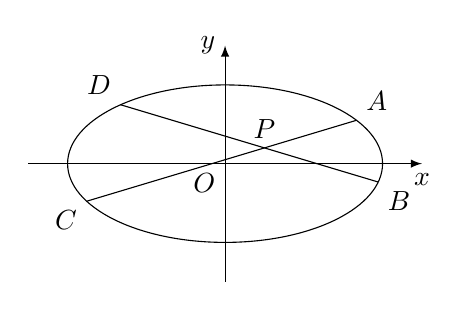
\begin{tikzpicture}[>=latex][scale = 1.5]
    \draw [->] (-2.5,0) -- (2.5,0) node [below] {$x$};
    \draw [->] (0,-1.5) -- (0,1.5) node [left] {$y$};
    \draw (0,0) node [below left] {$O$};
    \draw (0,0) ellipse (2 and 1);
    \draw (-1.3271,0.7481) node [above left] {$D$} -- (1.9447,-0.2334) node [below right] {$B$};
    \draw (-1.7575,-0.4773) node [below left] {$C$} -- (1.6693,0.5508) node [above right] {$A$};
    \draw (0.5,0.2) node [above] {$P$};
\end{tikzpicture}
\end{center}
